\documentclass[10pt]{article}

%% Various useful packages and commands from different sources

\usepackage[applemac]{inputenc}
\usepackage[english]{babel}
\usepackage[T1]{fontenc}
\usepackage{cite, url,color} % Citation numbers being automatically sorted and properly "compressed/ranged".
%\usepackage{pgfplots}
\usepackage{graphics,amsfonts}
\usepackage[pdftex]{graphicx}
\usepackage[cmex10]{amsmath}
% Also, note that the amsmath package sets \interdisplaylinepenalty to 10000
% thus preventing page breaks from occurring within multiline equations. Use:
 \interdisplaylinepenalty=2500
% after loading amsmath to restore such page breaks as IEEEtran.cls normally does.

% Compact lists
\usepackage{enumitem}
\usepackage{booktabs}
\usepackage{fancyvrb}

\usepackage{listings} % for Matlab code
\definecolor{commenti}{rgb}{0.13,0.55,0.13}
\definecolor{stringhe}{rgb}{0.63,0.125,0.94}
\lstloadlanguages{Matlab}
\lstset{% general command to set parameter(s)
framexleftmargin=0mm,
frame=single,
keywordstyle = \color{blue},% blue keywords
identifierstyle =, % nothing happens
commentstyle = \color{commenti}, % comments
stringstyle = \ttfamily \color{stringhe}, % typewriter type for strings
showstringspaces = false, % no special string spaces
emph = {for, if, then, else, end},
emphstyle = \color{blue},
firstnumber = 1,
numbers =right, %  show number_line
numberstyle = \tiny, % style of number_line
stepnumber = 5, % one number_line after stepnumber
numbersep = 5pt,
language = {Matlab},
extendedchars = true,
breaklines = true,
breakautoindent = true,
breakindent = 30pt,
basicstyle=\footnotesize\ttfamily
}

\usepackage{array}
% http://www.ctan.org/tex-archive/macros/latex/required/tools/
\usepackage{mdwmath}
\usepackage{mdwtab}
%mdwtab.sty	-- A complete ground-up rewrite of LaTeX's `tabular' and  `array' environments.  Has lots of advantages over
%		   the standard version, and over the version in `array.sty'.
% *** SUBFIGURE PACKAGES ***
\usepackage[tight,footnotesize]{subfigure}
\usepackage[top=2.2cm, bottom=2.2cm, right=1.7cm,left=1.7cm]{geometry}
\usepackage{indentfirst}


\setlength\parindent{0pt}
\linespread{1}

\usepackage{mathtools}
\DeclarePairedDelimiter{\ceil}{\lceil}{\rceil}
\DeclarePairedDelimiter{\floor}{\lfloor}{\rfloor}
\DeclareMathOperator*{\argmax}{arg\,max}
\newcommand{\M} {\mathtt{M}}
\newcommand{\dB} {\mathrm{dB}}
\newcommand{\tr} {\mathrm{tr}}



\graphicspath{ {figures/} }

% equations are numbered section by section
%\numberwithin{equation}{section}


\begin{document}
\title{Digital Transmission - Homework 2}
\author{Andrea Dittadi, Davide Magrin, Michele Polese}

\maketitle

\section*{Problem 1}

\subsection*{Choice of $N_h$}

In order to determine a suitable length $N_h$ of the impulse response, we consider the noise that we would introduce by performing the truncation of the power delay profile (that corresponds to a truncation of the random impulse response). The given discrete power delay profile of the channel is a sampled version of
\begin{equation}
\M(\tau) = \frac{1}{\bar{\tau}_{rms}} e^{-\tau / \bar{\tau}_{rms}}
\end{equation}
that is
\begin{equation}
\M(iT_C) = \frac{1}{\bar{\tau}_{rms}} e^{-iT_C / \bar{\tau}_{rms}}
\end{equation}
with $i$ non-negative integer and $T_C = 1$. This quantity must be then normalized in such a way that
\begin{equation}
\sum_{i=0}^{\infty} \M(iT_C) = 1 - C^2
\end{equation}
where $C = \sqrt{K / (K+1)}$ is the deterministic component of the first ray (for $i=0$) and $K$ is the Rice factor. Note that we are considering an infinite number of rays, but as a matter of fact MATLAB approximates as zero all values $\M(iT_C)$ for $i > 894$, therefore we stop the summation to 894 (actually 899, LOL). % TODO Do not forget to fix this

Knowing that the true impulse response of the channel has random properties described by the power delay profile $\M(iT_C)$ and by the quantity $C$, then we define the quality of the approximation due to truncation as
\begin{equation}
\Lambda_t(N_h) = \frac{E[||\mathbf{h}||^2]}{E[||\mathbf{\Delta h}||^2]} = \frac{C^2 + \sum_{i=0}^{\infty} \M(iT_C)}{\sum_{i=N_h}^{\infty} \M(iT_C)}
\end{equation}
where $\mathbf{h}$ is the vector of the impulse response $[h_0(nT_C),~h_1(nT_C),\ldots]$ and therefore
\begin{equation}
E[||\mathbf{h}||^2] = E[\sum_{i=0}^{\infty} |h_i(nT_C)|^2] = C^2 + \sum_{i=0}^{\infty} \M(iT_C).
\end{equation}
The noise in the system is
\begin{equation}
\Lambda = \frac{\M_x E[||\mathbf{h}||^2]}{4 \sigma_w^2} = \frac{\M_x (C^2 + \sum_{i=0}^{\infty} \M(iT_C))}{4 \sigma_w^2}
\end{equation}
where $\M_x$ is the statistical power of the input signal. Finally, we define the normalized ratio
\begin{equation}
\Lambda_n (N_h) = \frac{\Lambda_t}{\Lambda} = \frac{4 \sigma_w^2}{\M_x \sum_{i=N_h}^{\infty} \M(iT_C)} 
\end{equation}
to compare the noise of the system with the noise we are introducing by truncating $\M(iT_C)$ to $N_h$ samples.

Looking at the plot of $\Lambda_n (N_h)_{\dB}$ against $N_h$ in Fig.~\ref{fig:p01_lambda_n}, we can maintain that $N_h = 3$ is a good choice, since we have $\Lambda_n(2) \approx 2~\dB$ and $\Lambda_n(3) \approx 5.6~\dB$.

\begin{figure}[ht]
	\centering
	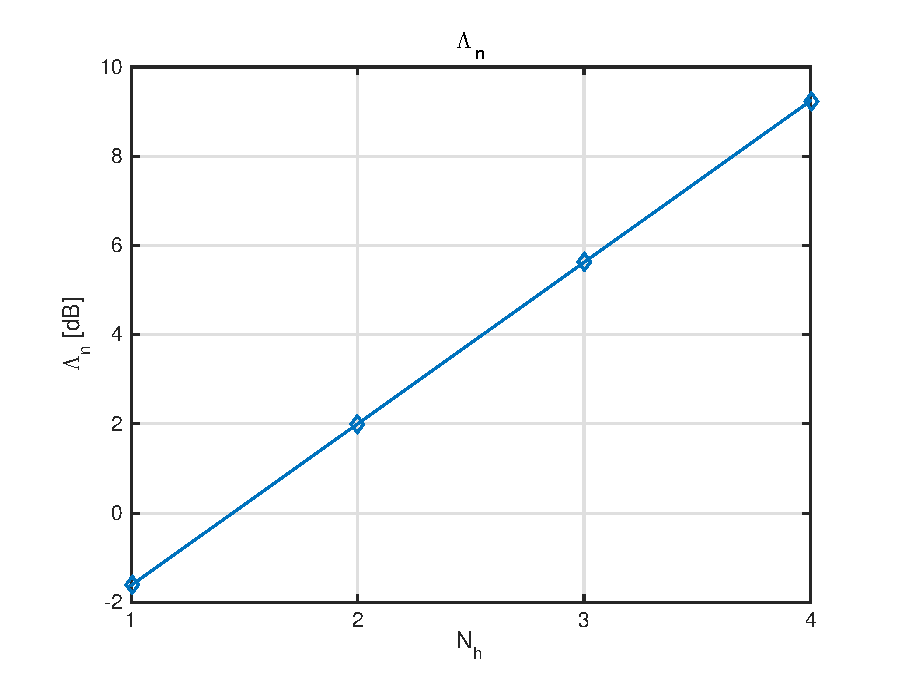
\includegraphics[width=0.52\textwidth]{p01_lambda_n}
	\caption{Plot of $\Lambda_n (N_h)$ in dB for the choice of $N_h$.}
    \label{fig:p01_lambda_n}
\end{figure}

\subsection*{Determine $E[|h_i(nTc)|^2]$}
Plot for $i = 0, 1, \dots, N_h - 1$ and put values in a table.

\subsection*{Show the behavior of $|h_i(nTc)|$}
Show the behavior for $n = 0, 1, \dots, 1999$.

\subsection*{Plot the histogram of $\frac{h_1}{\sqrt{E[|h_1|^2]}}$}
Plot the expected value based on values from 0 to 999.

\subsection*{Plot the histogram of $\frac{h_1(151Tc)}{\sqrt{E[|h_1(151Tc)|^2]}}$ for 1000 realizations}
Compare it with the theoretical result

\section*{Problem 2}

\subsection*{Setup of the receiver}
% TODO
Draw the polyphase implementation of the channel. This will help clarify what $N_i$ and $N$ are.

\begin{figure}[ht]
	\centering
	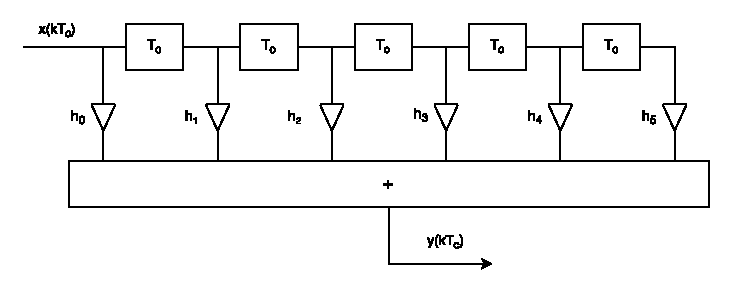
\includegraphics[width=0.75\textwidth]{channel_model}
	\caption{.}
    \label{fig:channel_model}
\end{figure}

\begin{figure}[ht]
	\centering
	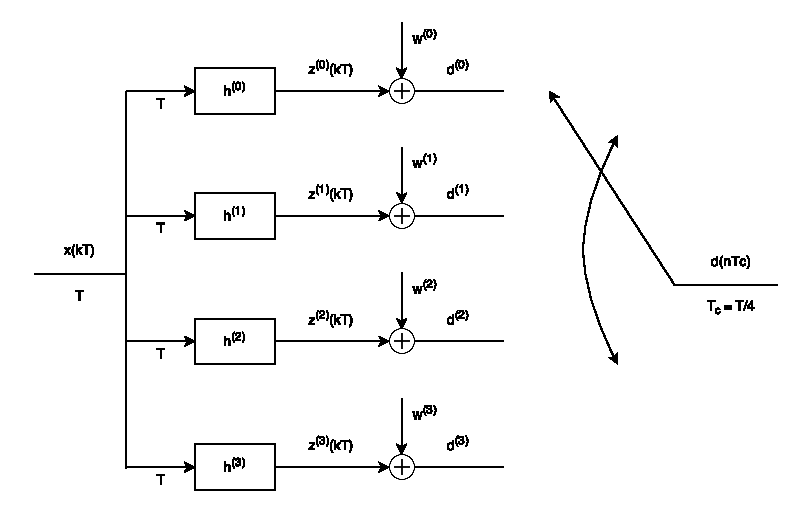
\includegraphics[width=0.75\textwidth]{polyphase}
	\caption{.}
    \label{fig:polyphase}
\end{figure}

At the receiver side, the LS method is used in order to estimate the impulse response of the channel. Assuming the number of coefficients of the channel is $N$, a partially repeated ML pseudo-noise sequence $x(kT)$ of periodicity $L$ and length $L + N_{max} - 1$ is sent through the channel, with $N_{max} = \max \{N_i\}$ and $N_i$ defined as above. In its polyphase implementation, the channel is a parallel of 4 filters with common input and sampling period $T$. In order to change the sampling period from $T$ to $T_C$, these branches are followed by a parallel/series switch that selects the outputs of the filters, passing to the next branch every $T_C$ seconds. This yields an output signal $d(nT_C)$ that is used by the receiver to estimate the coefficients $\mathbf{h}$ by $\mathbf{\hat{h}}$.

The actual estimation is performed separately on the 4 branches, each denoted by its index $i = 0,\ldots,3$, where for each branch we consider $d(kT+iT_C)$ as output, $\mathbf{h}_i = [h(iT_C), h(T+iT_C), \ldots, h((N_i-1)T + iT_C)]$ as impulse response, and $x(kT)$ is the input for all branches. Note that in the following we will always refer to the different polyphase branches with the index $i$, the dependance on time of the impulse response of the channel will be implied, and the notation
\begin{equation}\label{eq:def_ir_branch}
h_i(k) = h(kT+iT_C), k=0,\ldots,N_i-1
\end{equation}
will mean the $k$-th sample of the impulse response of the $i$-th branch, i.e. the impulse response of the channel at lag $(4k+i)T_C$.

The solution of the LS problem, for the estimation of the coefficients of the $i$-th polyphase branch, is given by
\begin{equation}
	\mathbf{\Phi}_i \mathbf{\hat{h}}_i = \boldsymbol\vartheta_i
\end{equation}
where $\mathbf{\Phi}_i$ is the autocorrelation $N_i \times N_i$ matrix of the input signal, $ \boldsymbol\vartheta_i$ is the cross-correlation vector between the input signal and the desired output (i.e. the output of the filter), and $\mathbf{\hat{h}}_i$ is the vector of the estimated coefficients for branch $i$. More precisely,
\begin{equation}
	\mathbf{\Phi}_i = [\Phi_i(j,n)] \quad \mathrm{ with } \quad \Phi_i(j,n) = \sum_{k=N_i-1}^{N_i-1+L-1} x^*(k-j)x(k-n), \quad j,n=0,\ldots,N_i-1
\end{equation}
\begin{equation}
	\boldsymbol\vartheta_i ^T = [\vartheta_i(0),\ldots, \vartheta_i(N_i-1)] \quad \mathrm{ with } \quad \vartheta_i(n) = \sum_{k=N_i-1}^{N_i-1+L-1} d(k)x^*(k-n).
\end{equation}

If $\mathbf{\Phi}_i^{-1}$ exists, i.e. $\mathbf{\Phi}_i$ is full rank, the LS solution is computed as
\begin{equation}
	\mathbf{\hat{h}}_i = \mathbf{\Phi}_i^{-1} \boldsymbol\vartheta_i.
\end{equation}
We note that the condition of $\mathbf{\Phi}_i$ being full rank requires that its dimension $N_i$ be at most equal to the periodicity $L$ of the ML sequence we are using. In fact, if $N_i > L$ we have
\begin{equation}
	\Phi_i(j+L, n) = \sum_{k=N_i-1}^{N_i-1+L-1} x^*(k-j-L)x(k-n) = \Phi_i(j, n), \quad n=0,\ldots,N_i-1, \quad j = 0,\ldots,N_i-1-L
\end{equation}
which means that there can only be $L$ independent rows or, equivalently, that the rank of $\mathbf{\Phi}_i$ is $\min \left\lbrace N_i, L \right\rbrace$. Therefore, if $N_i > L$ then the rank of $\mathbf{\Phi}_i$ is less than $N_i$ and $\mathbf{\Phi}_i^{-1}$ does not exist. In conclusion, this consideration places a bound on the number $N$ of coefficients of the overall system for the LS estimator, that is
\begin{equation}
	\left\lceil\frac{N}{4}\right\rceil = N_{max} \leq L.
\end{equation}

To compute the error function in the next section, we need the output of the system given by $\hat{\mathbf{h}}$, that is
\begin{equation}
	\hat{d}(kT_C) = \sum_{n=-\infty}^{+\infty} x(4nT_C)\hat{h}((k-4n)T_C).
\end{equation}
since $T/T_C=4$. If we split that equation in 4 polyphase components, and omit $T_C$, we can define
\begin{equation}
	\hat{d}_i(k) = \hat{d}(4k+i) = \sum_{n=-\infty}^{+\infty} x(4n)\hat{h}(4(k-n)+i) = \sum_{n=-\infty}^{+\infty} x(4n)\hat{h}_i(k-n),\quad i=0,\ldots,3
\end{equation}
where $\hat{h}_i(k) = \hat{h}(4k+i)$ is the estimated impulse response of the $i$-th branch, defined the same way as $h_i(k)$. Finally, if we consider $x$ at time instants that are multiples of $T$, we can drop the factor 4 and we have that the output $\hat{d}_i$ of a branch is, as expected, the following convolution:
\begin{equation}
	\hat{d}_i(k) = \sum_{n=-\infty}^{+\infty} x(n)\hat{h}_i(k-n) = x \ast \hat{h}_i (k) ,\quad i=0,\ldots,3.
\end{equation}

To perform this computation in matrix form, we define the $N_{max} \times (L+1)$ matrix
\begin{equation}
\mathbf{x}_T(k) =
 \begin{bmatrix}
  x(k-L) & x(k-L+1) & \cdots & x(k) \\
  x(k-L-1) & x(k-L) & \cdots & x(k-1) \\
  \vdots  & \vdots  & \ddots & \vdots  \\
  x(k-L-N_{max}+1) & x(k-L-N_{max}+2) & \cdots & x(k-N_{max}+1) \\
 \end{bmatrix}
\end{equation}
where we point out that if $N_{max} = 1$ then the ML sequence has length $L+N_{max}-1 = L$ and therefore we take $x(k-L), x(k-L-1), \ldots = 0$ by definition. We will see that this does not affect the result. If we define the polyphase impulse response matrix as the following $4\times N_{max}$ matrix
\begin{equation}
\mathbf{\hat{h}} =
 \begin{bmatrix}
  \mathbf{\hat{h}}_0 \\
  \vdots  \\
  \mathbf{\hat{h}}_3 \\
 \end{bmatrix} =
 \begin{bmatrix}
  \hat{h}(0) & \hat{h}(4+0) & \ldots & \hat{h}\left[4(N_{max}-1) + 0\right] \\
  \vdots  & \vdots  & \ddots & \vdots  \\
  \hat{h}(3) & \hat{h}(4+3) & \ldots & \hat{h}\left[4(N_{max}-1) + 3\right]\\
 \end{bmatrix}
\end{equation}
then we can derive the output of the system $\hat{\mathbf{h}}$ as
\begin{equation}
	\hat{\mathbf{d}} = \hat{\mathbf{h}} \; \mathbf{x}_T.
\end{equation}

In this output matrix evaluated at time $k$, the element with row index $i$ and column index $L-j$ is
\begin{equation}
	\hat{d}^{(k)}(i, L-j) = \sum_{n=0}^{N_{max}-1} \hat{h}_i(n) x(k-n-j) =  \sum_{n=-\infty}^{+\infty} \hat{h}_i(n) x(k-n-j) =  \sum_{n=-\infty}^{+\infty} x(n) \hat{h}_i(k-n-j) = \hat{d}_i(k-j)
\end{equation}
with $i=0,\ldots,3,\; j=0,\ldots,L$. The full $4 \times (L+1)$ matrix at time $k$ can now be written as
\begin{equation}
\hat{\mathbf{d}}(k) =
 \begin{bmatrix}
  \hat{d}_0(k-L) & \hat{d}_0(k-L+1) & \cdots & \hat{d}_0(k) \\
  \vdots  & \vdots  & \ddots & \vdots  \\
\hat{d}_3(k-L) & \hat{d}_3(k-L+1) & \cdots & \hat{d}_3(k) \\
 \end{bmatrix}
\end{equation}
and contains the last $4(L+1)$ values of the output $\hat{d}$ up to the time instant $kT+3T_C$. Recalling the definition in (\ref{eq:def_ir_branch}), that applies to $\hat{\mathbf{h}}$ as well, we can concatenate vertically all rows, from the left to the right, to obtain the vector
\begin{equation}
	\hat{\mathbf{d}}' (k) = \left[\hat{d}[(k-L)T],\; \hat{d}[(k-L)T + T_C], \ldots,\; \hat{d}[kT + 3T_C] \right]
\end{equation}

The transient of the whole system is $N-1$ samples long, if we consider the $T_C$ sampling period. However, after $N-1-(T/T_C - 1) = N-4$ samples we have already discarded all past samples of the signal $x$: we are still considering 3 initial conditions on $x$, but they do not contain samples of the signal, since it is defined with a sampling period equal to $4T_C$, thus they do not affect the output and we do not consider them as transient. Note that if $N \leq 4$ we do not need to discard any sample, therefore we define the number of samples of the transient in the $T_C$ domain as $N_{tr} = \max \{0, N-4\}$.

The signal $x$ has $L+N_{max}-1$ samples, and we are now considering $L+1$ samples, which means that we are disregarding $N_{max}-2$ samples in the $T$ domain, that correspond to $4(N_{max}-2)$ samples of $\hat{d}$. We still need to discard $N_{tr} - 4(N_{max}-2) = \max \{ 0, N-4 \} - 4 \ceil{N/4} + 8$ samples of $\hat{d}$. Note that this also works with $N \leq 4$. In this case, $x$ has length $L$ and we need to keep all output samples, that is to say the transient is actually 0. This algorithm takes the whole signal $x$ with a 0 at the front, $\hat{\mathbf{h}}$ is a column vector, and the first column of $\hat{\mathbf{d}}$ is all zeros. While this first column is useless, the second one has to be entirely kept. According to the expression above, the number of samples that need to be discarded is indeed 4.


\subsection*{Determine $L$ and $N$}

For each considered pair $(L,N)$, we run 100 (TODO) simulations in which we take subsequent disjoint time interval of the time-varying channel, evaluate its output $d(nT_C)$, compute an LS estimate of $\mathbf{h}_i \; \forall i$, and compute the error function defined as
\begin{equation}
	\mathcal{E} = \sum 
\end{equation}

\subsection*{Estimate of $E[||\mathbf{\hat{h}}-\mathbf{h}||^2]$ assuming $\mathbf{h}$ is known}

\subsection*{Comparing the estimate of $E[||\mathbf{\hat{h}}-\mathbf{h}||^2]$ with its theoretical value}

We can now give a theoretical value of the estimation error yielded by this implementation of the LS method. It is the average error on the estimate of the impulse response $\mathbf{h}$ if we assume that we are using $N$ coefficients, $L$ input samples of the ML sequence, and that $N=N_h$. Formally, the estimation error is given by
\begin{equation}
	E[||\mathbf{\hat{h}}-\mathbf{h}||^2] = E[||\mathbf{\Delta h}||^2] = E[\sum_{i=0}^{3} ||\mathbf{\Delta h}_i||^2] = \sum_{i=0}^{3} E[||\mathbf{\Delta h}_i||^2]
\end{equation}
where we split the formula according to the 4 branches of the polyphase implementation. Following the rationale presented in \cite{bc}, for each branch with index $i=0,\ldots,3$ we get
\begin{equation}
	\mathbf{\Phi}_i^{-1} = \frac{1}{L+1} \left( \mathbf{I} + \frac{\mathbf{1}_{N_i \times N_i}}{L+1-N_i} \right)
\end{equation}
where $\mathbf{1}_{N_i \times N_i}$ is the $N_i \times N_i$ matrix with all elements equal to $1$, and therefore
\begin{equation}
	\tr [\mathbf{\Phi}_i^{-1}] = \frac{N_i(L+2-N_i)}{(L+1)(L+1-N_i)}.
\end{equation}
Finally, we can express the estimation error of the $i$-th branch as
\begin{equation}
	E[||\mathbf{\Delta h}_i||^2] = \sigma_w^2 \; \tr [(\mathbf{\Phi}_i^*)^{-1}] = \sigma_w^2 \; \tr [\mathbf{\Phi}_i^{-1}] = \sigma_w^2 \frac{N_i(L+2-N_i)}{(L+1)(L+1-N_i)}
\end{equation}
where $\mathbf{\Phi}_i$ is Hermitian. Going back to the overall estimation error we have
\begin{equation}
	E[||\mathbf{\hat{h}}-\mathbf{h}||^2] = \sum_{i=0}^{3} E[||\mathbf{\Delta h}_i||^2] = \frac{\sigma_w^2}{L+1} \sum_{i=0}^{3} \frac{N_i (L+2-N_i)}{L+1-N_i}.
\end{equation}

Now we are ready to compare the empirical estimation error measured in the previous section, with its theoretical value we just derived. With $L$ fixed, the estimation error becomes worse as $N$ increases, but of course this holds for $N \geq N_h$ only, otherwise this result does not apply. In fact, when estimating $\mathbf{h}$ with $N<N_h$ the actual error becomes larger since we have less degrees of freedom with respect to the ones of the system. On the other hand, when $N > N_h$ it is as though we were estimating a channel with $N_h = N$ in which the last $N_h - N$ coefficients are zero. Therefore, of course the estimation error gets worse -- because we are performing more estimations and all of them are subject to error -- but it makes no difference whether or not the additional $N_h - N$ coefficients are indeed zero. For this reason, the empirical estimation error follows the theoretical value for $N \geq N_h$, as shown in Fig.~\ref{fig:p02_comparetheoreticaldeltah}.

\begin{figure}[ht]
	\centering
	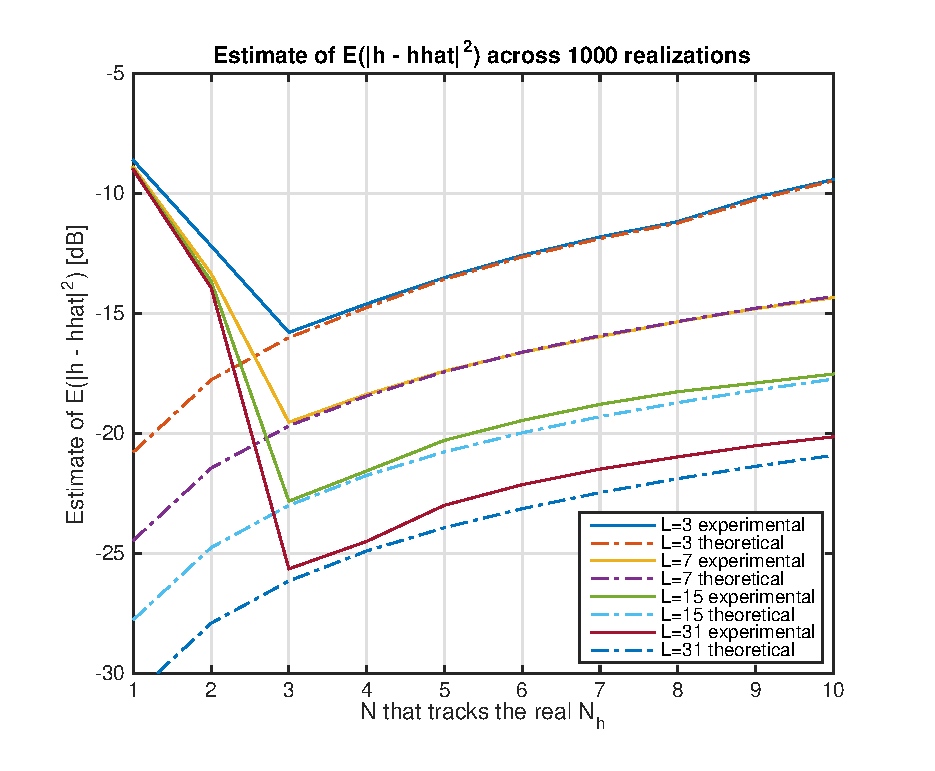
\includegraphics[width=0.75\textwidth]{p02_comparetheoreticaldeltah}
	\caption{Experimental estimation error $E[||\mathbf{\Delta h}||^2]$ with different values of $L$ and $N$, compared with its theoretical value.}
    \label{fig:p02_comparetheoreticaldeltah}
\end{figure}


\begin{thebibliography}{10}

\bibitem{bc}
Benvenuto, Cherubini, Algorithms for Communications Systems and their Applications, Wiley, 2004


\end{thebibliography}

\end{document}
